\documentclass[12pt, letterpaper]{article}
\usepackage{graphicx} % Required for inserting images
\usepackage{hyperref}
\usepackage{listings}
\usepackage{amssymb}
\usepackage{amsmath}
\usepackage[english]{babel}
\usepackage{nicefrac, xfrac}
\usepackage{mathtools}
\newcommand{\acc}{\\\hphantom{}\\}
\usepackage[table,xcdraw]{xcolor}
\usepackage[paper=a4paper,left=20mm,right=20mm,bottom=25mm,top=25mm]{geometry}
\renewcommand{\labelenumii}{\arabic{enumi}.\arabic{enumii}}
    \renewcommand{\labelenumiii}{\arabic{enumi}.\arabic{enumii}.\arabic{enumiii}}
    \renewcommand{\labelenumiv}{\arabic{enumi}.\arabic{enumii}.\arabic{enumiii}.\arabic{enumiv}}
\title{Impiegati e Studenti (gruppo 42)}
% \author{ Giacomo Biribicchi \and Marco Casu \and Christian Di Manno \and Alessandro Gautieri }
\date{}


\begin{document}

\maketitle


\section{Requisiti}
\begin{enumerate}
    \item \textbf{Persona}\begin{enumerate}
        \item nome 
        \item cognome 
        \item codice fiscale 
        \item data di nascita
        \item Sesso \begin{enumerate}
        \item Uomo \begin{enumerate}
            \item posizione militare - il ruolo che l'uomo assume nell'esercito
        \end{enumerate}
        \item Donna \begin{enumerate}
            \item maternità - il numero di figli
        \end{enumerate}
    \end{enumerate}
    \item Impiego\begin{enumerate}
        \item stipendio in euro
        \item Ruolo\begin{enumerate}
            \item segretario 
            \item direttore 
            \item progettista - insieme ai progetti di cui è responsabile.
        \end{enumerate}
    \end{enumerate}
    \item Studente \begin{enumerate}
        \item matricola
    \end{enumerate}
    \end{enumerate}
    \item\textbf{Progetto} \begin{enumerate}
        \item nome
    \end{enumerate}
\end{enumerate}
\newpage
\section{Documenti di Specifica}
\subsection{Tipi di Dato}
I tipi sono dati sottoforma di espressioni regolari : \acc
CF = [A-Z]\{6\} [0-9]\{2\} [A-Z]\{1\} [0-9]\{2\} [A-Z]\{1\} [0-9]\{3\} [A-Z]\{1\}

\section{UML}\begin{center}
    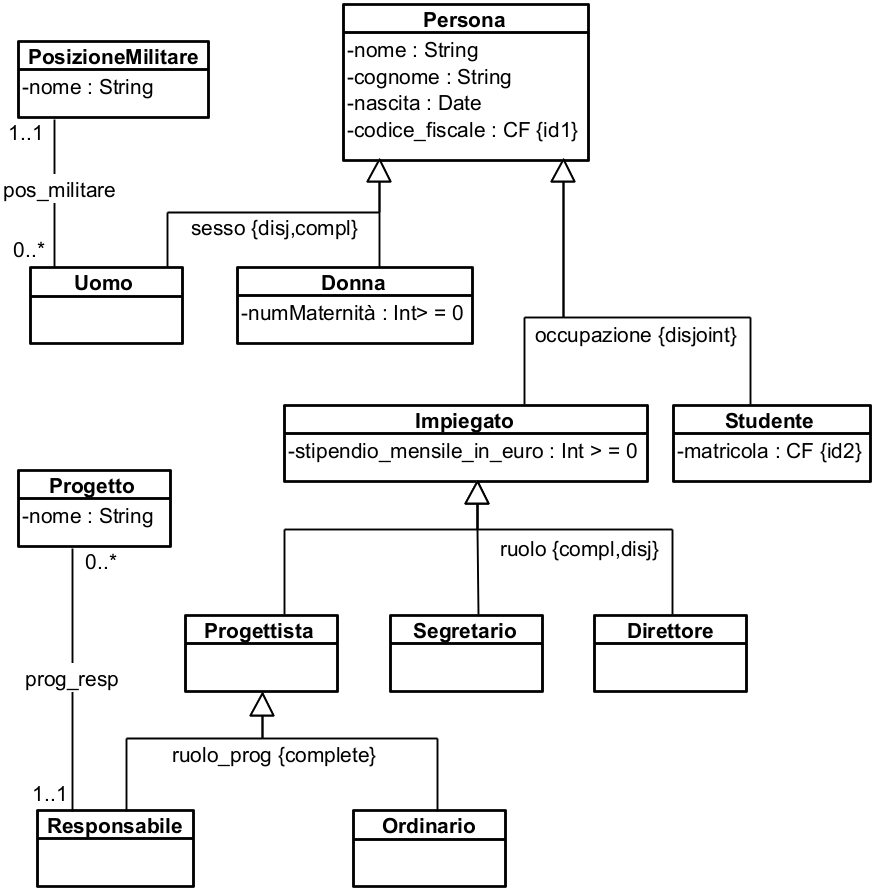
\includegraphics[width=\textwidth]{images/UML.png}
\end{center}

\end{document}

